% =====================================================================
% Fig.5 -- Per-token routing-confidence distribution x^s = max_m S_{n,m}.
% outline.md §3.6 (routing interpretability) / traceability C3 ("x_scores 分布").
% Self-contained pgfplots figure; \input into the paper.
% Requires in preamble: \usepackage{pgfplots}\pgfplotsset{compat=1.16}
%
% DATA PROVENANCE (verbatim, no fabrication):
%   fig58_assets/fig5_{Urban100,Manga109}_xscore_hist.csv produced on the
%   training machine by CATANet/scripts/build_routing_figures.py with the x4
%   model net_g_250000, accumulating x^s over ALL LR images of each test set
%   (Urban100: 4,839,460 tokens/block; Manga109: 6,545,996 tokens/block).
%   Curves below are the normalized frequency (% of tokens per 0.02 bin) for
%   three representative blocks b0 (M=16), b2 (M=64), b3 (M=128). Uniform
%   floor 1/M shown as dotted vertical lines (b0: 0.0625, b2: 0.0156,
%   b3: 0.0078). Per-block stats in fig5_*_xscore_stats.csv: block-mean x^s
%   sits at ~1.5-1.9x the floor (e.g. Urban100 b0 0.1093 vs 0.0625, b3 0.0124
%   vs 0.0078), i.e. informative but soft assignment. >99.8% of mass lies in
%   [0,0.30], so the x-axis is clipped there for readability.
% =====================================================================
\begin{figure}[t]
\centering
\pgfplotsset{
  xscoreaxis/.style={
    width=\linewidth, height=4.2cm,
    xmin=0, xmax=0.30, ymin=0, ymax=100,
    ytick={0,25,50,75,100},
    xlabel={routing confidence $x^{\mathrm{s}}=\max_m S_{n,m}$},
    ylabel={tokens (\%)},
    ymajorgrids, grid style={gray!22},
    tick label style={font=\scriptsize},
    label style={font=\footnotesize},
    legend style={font=\scriptsize, at={(0.97,0.95)}, anchor=north east,
                  draw=none, fill=white, fill opacity=0.7, text opacity=1,
                  row sep=-1pt},
    title style={font=\footnotesize, yshift=-4pt},
  },
}
\begin{minipage}{\linewidth}
\centering
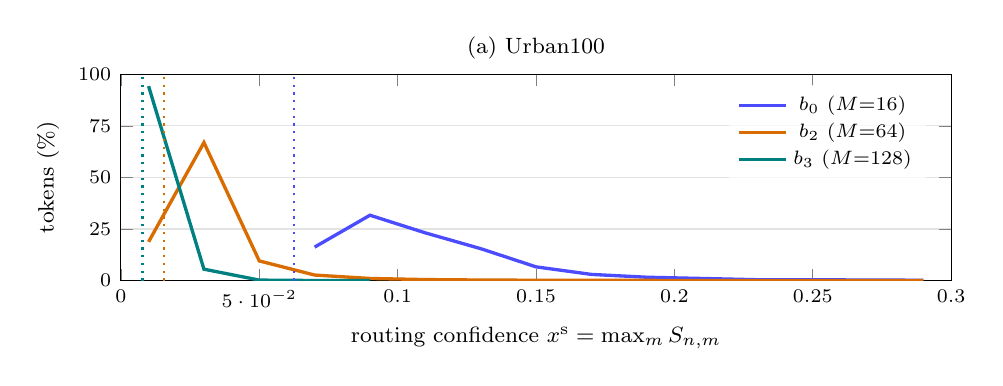
\begin{tikzpicture}
\begin{axis}[xscoreaxis, title={(a) Urban100}]
\addplot[draw=blue!70, very thick] coordinates {
  (0.07,16.2111) (0.09,31.6671) (0.11,23.1137) (0.13,15.4588) (0.15,6.6313)
  (0.17,2.9667) (0.19,1.5974) (0.21,0.9969) (0.23,0.397) (0.25,0.3825)
  (0.27,0.2386) (0.29,0.1443) };
\addplot[draw=orange!85!black, very thick] coordinates {
  (0.01,18.7685) (0.03,66.9281) (0.05,9.506) (0.07,2.6561) (0.09,1.0022)
  (0.11,0.4613) (0.13,0.2415) (0.15,0.1404) (0.17,0.089) (0.19,0.0578)
  (0.21,0.0375) (0.23,0.0282) (0.25,0.02) (0.27,0.015) (0.29,0.0116) };
\addplot[draw=teal, very thick] coordinates {
  (0.01,94.2813) (0.03,5.4999) (0.05,0.2043) (0.07,0.0134) (0.09,0.0009) };
\draw[blue!70, dotted, thick] (axis cs:0.0625,0) -- (axis cs:0.0625,100);
\draw[orange!85!black, dotted, thick] (axis cs:0.0156,0) -- (axis cs:0.0156,100);
\draw[teal, dotted, thick] (axis cs:0.0078,0) -- (axis cs:0.0078,100);
\legend{$b_0$ ($M{=}16$), $b_2$ ($M{=}64$), $b_3$ ($M{=}128$)}
\end{axis}
\end{tikzpicture}
\end{minipage}

\vspace{2pt}
\begin{minipage}{\linewidth}
\centering
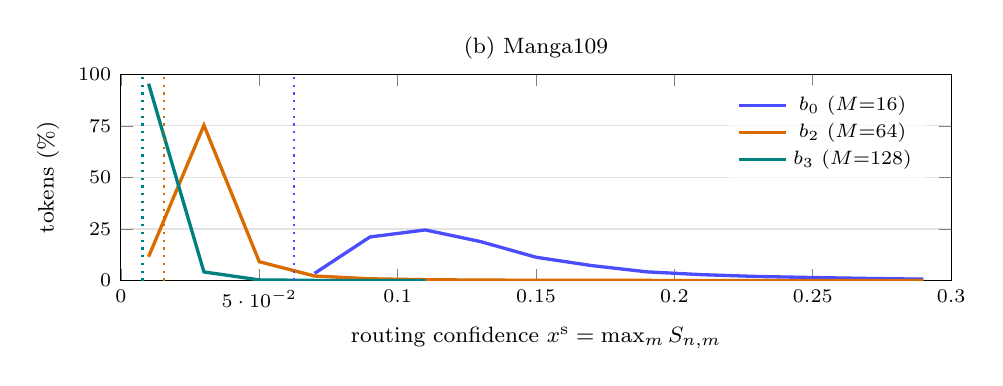
\begin{tikzpicture}
\begin{axis}[xscoreaxis, title={(b) Manga109}]
\addplot[draw=blue!70, very thick] coordinates {
  (0.07,3.4849) (0.09,21.1291) (0.11,24.5368) (0.13,18.8673) (0.15,11.2919)
  (0.17,7.2655) (0.19,4.2136) (0.21,2.8329) (0.23,1.9641) (0.25,1.4542)
  (0.27,1.009) (0.29,0.6623) };
\addplot[draw=orange!85!black, very thick] coordinates {
  (0.01,11.53) (0.03,75.3017) (0.05,9.1121) (0.07,2.1833) (0.09,0.8387)
  (0.11,0.4047) (0.13,0.2143) (0.15,0.1256) (0.17,0.0812) (0.19,0.0557)
  (0.21,0.0398) (0.23,0.0267) (0.25,0.018) (0.27,0.0139) (0.29,0.0107) };
\addplot[draw=teal, very thick] coordinates {
  (0.01,95.4593) (0.03,4.1735) (0.05,0.3019) (0.07,0.051) (0.09,0.011)
  (0.11,0.0025) };
\draw[blue!70, dotted, thick] (axis cs:0.0625,0) -- (axis cs:0.0625,100);
\draw[orange!85!black, dotted, thick] (axis cs:0.0156,0) -- (axis cs:0.0156,100);
\draw[teal, dotted, thick] (axis cs:0.0078,0) -- (axis cs:0.0078,100);
\legend{$b_0$ ($M{=}16$), $b_2$ ($M{=}64$), $b_3$ ($M{=}128$)}
\end{axis}
\end{tikzpicture}
\end{minipage}
\caption{Distribution of the per-token routing confidence
$x^{\mathrm{s}}=\max_m S_{n,m}$ (Eq.~\eqref{eq:belong}) at $\times4$, accumulated
over \emph{all} test images of (a)~Urban100 and (b)~Manga109 with the final model.
Curves are shown for three representative TAB blocks with increasing prototype
count $M$; dotted vertical lines mark the uniform-assignment floor $1/M$. In every
block the distribution sits clearly to the right of its floor (block-mean
$\approx 1.5$--$1.9\times\,1/M$) yet stays far from $1$, confirming that the softmax
assignment is \emph{informative but soft}: tokens commit to a prototype more than
chance while retaining the graded confidence that the C3 components
(ordering key, IASA gate, soft fallback) rely on. As $M$ grows the mode shifts
toward the (lower) floor, consistent with confidence being spread over more slots.}
\label{fig:xscore_hist}
\end{figure}
